\section{Device Configuration}

Abstractly, the IOMMU uses a set of table structure to configure address translation
for individual devices. This table structure is collectively referred to as the
\textit{Device Tables}.

It is up to the implementation to determine whether the device tables are memory-resident
or stored in special registers provided by the IOMMU. When the device tables are stored in
specialized registers, the registers should be MMIO register and the MMIO registers should
reside in the register MMIO range of the IOMMU. In this case, the register \dtbase\ is not
defined.

Each IOMMU is associated with a \textit{domain} which consists of the devices whose DMA
requests is translated by this IOMMU. Each device within the same domain is assigned a
unique identifier, typically by the peripheral bus. The identifier is used to tag the relevant
memory requests originated from that device. Upon receiving the memory requests, the IOMMU
looks up in the device tables using the identifier and retrieve the configuration for that
device.

The identifier for the incoming translation requests is termed a Requester Source ID
(RSID). The length of the RSID is \rsidlen.

\subsection{Source Identification}

The RSID is split into two parts for use in the device table look-up, RISDHI and
RSIDLO. The MMIO register called \rsiddiv\ specifies the split point. When \rsiddiv\ stores
value $N$, RSIDLO is RSID[$N-1$:$0$] and RSIDHI is RSID[$\rsidlen - 1$, $N$]. The
\rsiddiv\ register is \warl, an implementation can hardwire this register to a fixed
value. When \rsiddiv is zero, RSIDHI equals RSID and RSIDLO is not defined.

The \rsidlen\ is implementation defined. It should be at least such a length so that it is
capable to contain the all the IDs of the bus that the IOMMU is intended to work with.

\note The RSID corresponds to the identification in the bus that it is interfaced with.
For example, the AXI bus assigns an ID to each device, and each device is capable of
generating transactions of possibly multiple IDs. The concatenated ID is the RSID. In this
case the RSID should be at least as long as the concatenated ID.\noteend

\note In the case of AXI, the RSID is not the transaction ID. \noteend


\subsection{Device Table}
\label{sec:dev_tbl}

\subsubsection{Memory Resident Device Table}
\label{sec:mem_dt}

The device tables are 8-byte aligned arrays of 8-byte aligned entries called
\textit{device table entries}.

When \rsiddiv\ is not zero, there are two levels of device tables. The level-1 device
tables are indexed by RSIDHI, and the level-2 device tables are indexed by RSIDLO. The
level-1 device table entries contains the base address of the corresponding level-2 device
table. The level-2 device table entries point to \textit{translation descriptors} for that
device with the RSID that leads to the entry.  The translation descriptor contains the
base address of the top level page table and other control bits.

When \rsiddiv\ is zero, there is only one level of device table index by RSID. The entries
point to the translation descriptor for that device with the RSID.

If the IOMMU implements the memory resident device table support, it provides an
MMIO register called \dtbase\ that holds the 8-byte aligned physical address of the
level-1 device table in the memory. The \dtbase\ register resides in the register MMIO
range.

The \dtbase\ register is defined in Figure \ref{fig:dtbase_reg}. 

\begin{figure}[h!t]
    \begin{center}
        \begin{tabular}{@{}Jc@{}F}
    \instbitrange{63}{3} &
    \instbitrange{2}{0} \\
    \hline
    \multicolumn{1}{|c|}{Addr} &
    \multicolumn{1}{c| }{Reserved} \\
    \hline
    61 & 3 \\

    \end{tabular}
    \end{center}

    \caption{dtbase Register}
    \label{fig:dtbase_reg}
\end{figure}

The Addr field store the 8-byte aligned physical address of the level-1 device table.

When \rsiddiv\ is not zero, the device tables are multi-level structures. The level-1
device table contains $2^{RSIDHI}$ entries that points to level-2 tables. The level-1
device table is index by RSIDHI derived from the RSID. The level-1 device table entries
are defined in Figure \ref{fig:lv1_dt_entry}.

\begin{figure}[h!t]
    \begin{center}
        \begin{tabular}{@{}Jc@{}F}
    \instbitrange{63}{3} &
    \instbitrange{2}{0} \\
    \hline
    \multicolumn{1}{|c|}{Addr} &
    \multicolumn{1}{c| }{Reserved} \\
    \hline
    61 & 3 \\

    \end{tabular}
    \end{center}

    \caption{Level-1 Device Table Entry}
    \label{fig:lv1_dt_entry}
\end{figure}

The Addr field store the 8-byte aligned physical address of the level-2 device table.

The Reserved bits must be zero, otherwise the IOMMU raises a fault.

The level-2 device tables are 8-byte aligned tables indexed by RSIDLO. Each table contains
$2^{RSIDLO}$ entries that points to an extended device table. The level-2 device table
entries are defined in Figure \ref{fig:lv2_dt_entry}.

\begin{figure}[h!t]
    \begin{center}
        \begin{tabular}{@{}Jc@{}I@{}I@{}I}
    \instbitrange{63}{3} &
    \instbit{2} &
    \instbit{1} &
    \instbit{0} \\
    \hline
    \multicolumn{1}{|c|}{Addr} &
    \multicolumn{1}{c| }{F} &
    \multicolumn{1}{c| }{S} &
    \multicolumn{1}{c| }{V} \\
    \hline
    61 & 1 & 1 & 1 \\

    \end{tabular}
    \end{center}

    \caption{Level-2 Device Table Entry}
    \label{fig:lv2_dt_entry}
\end{figure}

The Addr field store the 8-byte aligned address of the translation descriptor.

The V bit controls if the address translation is enabled for the particular device
identified by the RSID. If V bit is set, the address translation is in effect i.e. the
address in the transaction from the originating device is subject to translation. If V bit
is clear, the address translation for that device is turned off, i.e. the IOMMU forwards
the address as-is.

The S bit (which stands for the Second stage) controls whether the device whose RSID leads to
the level-2 device table entry is subject to two-stages of address translation. If S bit
is set, it is subjected to two-stages of translation. If S bit is clear, it is only
subject to one-stage of translation.

The F bit (which stands for the First stage) controls whether the device whose RSID leads
to the level-2 device table entry is subject to stage-one address translation. If F bit is
set, stage-one address translation is enabled. If F bit is cleared, stage-one address
translation is disabled, i.e., the address in the DMA transaction is used only with
stage-two address translation.

When \rsiddiv\ is zero, there is only one level of device table. The entries in the
level-1 device table are the same as the level-2 device table when \rsiddiv\ is not zero.

\subsubsection{Register-based Device Table}

If the device tables are implemented as MMIO registers, the IOMMU provides $2^\rsidlen$ number
of registers called \dte[$x$], where $0 <= x <= 2^\rsidlen - 1$. The format of the register is
shown in Figure \ref{fig:dtex}. 
The upper bits
beyond the width of the physical address on the hardware platform can be ignored.

The IOMMU does not support stage-two translation if the device tables are implemented as
MMIO registers.

\begin{figure}[h!t]
    \begin{center}
        \begin{tabular}{@{}J@{}I@{}I}
    \instbitrange{63}{2} &
    \instbit{1} &
    \instbit{0} \\
    \hline
    \multicolumn{1}{|c|}{Addr} &
    \multicolumn{1}{c| }{P} &
    \multicolumn{1}{c| }{V} \\
    \hline
    61 & 1 & 1 \\

    \end{tabular}
    \end{center}

    \caption{Device Table Entry Implemented as MMIO Register}
    \label{fig:dtex}
\end{figure}

The Addr field stores the base address of the top level address table for the device with
the RSID. The P bit indicates the fault reporting mode of the device. If P bit is set, the
IOMMU suspend the in-flight transaction that caused a fault. If P bit is cleared, the
IOMMU terminates the transaction immediately. 

If the V bit is set, the device table entry is valid. Otherwise, the entry is invalid.

The \dte[$x$] registers reside in a dedicated 4K-aligned region called device table range.

The IOMMU uses the content of \dte[$x$] for the device with RSID value $x$ to get the
address of the translation descriptor. The IOMMU zero-extend the content of the \dte[$x$]
registers to generate the address of the translation descriptor.

In this case, the \dtbase\ register is not defined.

\subsection{Translation Descriptor}
\label{sec:trans_desc}

The translation descriptor contains the root address of the address tables. There are
three parts in the descriptor, two of which corresponding to one translation stage.

The translation descriptor format is shown in Table \ref{tbl:dev-tbl-bits}:

\begin{table}[h!t]
    \centering
    \begin{tabular}{ | l | l | }

    \hline
    Bit 0 - 63   & Stage One Control \\
    \hline
    Bit 64 - 127 & Stage Two Control \\
    \hline
    Bit 128 - 191 & Device Configuration \\
    \hline

    \end{tabular}
    \caption{Bits in Translation Descriptor}
    \label{tbl:dev-tbl-bits}
\end{table}


Each translation descriptor specifies the base address of the first and the second stage
of translation tables. If two-stage translation is not implemented, it is recommended that
the stage-two bits are set to zeros. 

\begin{figure}[ht!]

    \begin{center}
        \begin{tabular}{@{}S@{}Y@{}T@{}K}
    \instbitrange{127}{124} &
    \instbitrange{123}{122} &
    \instbitrange{121}{108} &
    \instbitrange{107}{64} \\
    \hline
    \multicolumn{1}{|c|}{S2MODE} &
    \multicolumn{1}{ c|}{Reserved} &
    \multicolumn{1}{ c|}{VMID} &
    \multicolumn{1}{ c|}{S2PPN} \\
    \hline
    4 & 2 & 14 & 44 \\
    \end{tabular}
    \end{center}

    \caption{Stage Two Control Field in Translation Descriptor}
    \label{fig:stage-two-bits-in-dev-tbl-entry}
\end{figure}

Bits 64-127 are adapted from the format of the RV64 \textit{hgatp} CSR, with bits 123 -
122 currently reserved. The S2MODE field is the same as the RV64 \textit{hgatp} CSR's MODE
field. All the modes are supported.  The Reserved bits must be zero, otherwise the IOMMU
raises a fault. If the S bit is set in the device table entry that leads to a translation
descriptor, and the S2MODE is zero, the IOMMU raises a fault.

The format of the stage-two bits is shown in Figure
\ref{fig:stage-two-bits-in-dev-tbl-entry}. The S2PPN field is the same as the PPN field in
\textit{hgatp}. 

The S2MODE field determines if stage-two translation is enabled. And if it is, which
translation mode is effective. Its value should be consistent with the S bit in the device
table entry that points to this translation descriptor. Otherwise, the IOMMU raises a
fault.

When the S2MODE field is zero, bits 0-63 contains the 4K-aligned physical address of the
first stage address table. Its format is adapted from the RV64 \textit{satp} CSR as shown
in Figure \ref{fig:stage-one-bits-s2mode-zero}.

The Reserved bits must be zero, otherwise the IOMMU raises a fault.

\begin{figure}[ht!]

    \begin{center}
        \begin{tabular}{@{}S@{}N@{}K}
    \instbitrange{63}{60} &
    \instbitrange{59}{44} &
    \instbitrange{43}{0} \\
    \hline
    \multicolumn{1}{|c|}{S1MODE} &
    \multicolumn{1}{ c|}{ASID} &
    \multicolumn{1}{ c|}{S1PPN} \\
    \hline
    4 & 16 & 44 \\
    \end{tabular}
    \end{center}

    \caption{Stage One Control Field}
    \label{fig:stage-one-bits-s2mode-zero}
\end{figure}

If the S2MODE field is not zero, bits 0-63 contains the 4K-aligned physical page number of
the stage-one address table page allocated by the guest VM. The format remain the same.
The Reserved bits must be set to zero, otherwise the IOMMU reports a fault.

%\note The register MMIO page can be hidden from the guest VM if the hypervisor intends to
%enforce only the second stage of translation. \noteend

%If the S2MODE field is not zero, bits 128-191 records the RSID used during the nested
%address translation. The device identifier presented to the guest VM might be different
%from the identifier used by the host, therefore, this field allows the host to override
%the RSID for the guest.

%\begin{figure}[ht!]
%
%    \begin{center}
%        \begin{tabular}{@{}T@{}K}
%        \instbitrange{63}{44} &
%        \instbitrange{43}{0} \\
%        \hline
%        \multicolumn{1}{|c|}{Reserved} &
%        \multicolumn{1}{ c|}{RPAddr} \\
%        \hline
%        20 & 44 \\
%        \end{tabular}
%    \end{center}
%
%    \caption{Stage One Control Field When S2MODE is not Zero}
%    \label{fig:stage-one-bits-in-dev-tbl-entry}
%\end{figure}

\note When the IOMMU is active, i.e. \iommucapen.E = 1, the system software can set both
S1MODE and S2MODE to zero to let a device access memory effectively with physical
addresses. This configuration is functionally valid, however, it is not recommended since
it leads to degraded performance. \noteend

Bits 128 to 191 are the configuration bits for the device whose RSID leads to this
descriptor. Its format is shown in Table \ref{tbl:desc_conf}.

\begin{table}[h!t]
    \centering
    \begin{tabular}{ | l | l | }

    \hline
    Bit 0 - 1  &  Device Table Walk Fault Configuration \\
    \hline
    Bit 2 - 3  &  Host Address Table Walk Fault Configuration \\
    \hline
    Bit 4 - 5  &  Hypervisor Overrides \\
    \hline

    \end{tabular}
    \caption{Configuration Bits in Translation Descriptor}
    \label{tbl:desc_conf}
\end{table}

Bits 0 - 1 controls the behavior of the IOMMU during device table walk. Table
\ref{tbl:dev_tbl_walk_conf} shows the meaning of the values.

\begin{table}[h!t]
    \centering
    \begin{tabular}{ | l | l | }

    \hline
    Value  &  IOMMU Behavior  \\
    \hline
    00b  &  Pause mode, IOMMU withholds the transaction, no response is sent to the initiating device  \\
    \hline
    01b &   Abort mode, IOMMU responds with error with no data  \\
    \hline
    10b &   Abort mode, IOMMU responds with all zeros to reads, ignores writes  \\
    \hline
    11b &   Abort mode, IOMMU responds with all ones to reads, ignores writes  \\
    \hline

    \end{tabular}
    \caption{Device Table Walk Fault Configuration}
    \label{tbl:dev_tbl_walk_conf}
\end{table}

If one-stage translation is configured for a device, bits 2 - 3 of the configuration bits
in the translation descriptor controls the behavior of the IOMMU during the address table
walk. If two-stage translation is configured, these bits control the address table walk
for in the second stage. The encoding is shown in Table \ref{tbl:addr_tbl_walk_conf}.

\note Some simple systems may not need dynamic DMA page support, these systems can simply
pre-allocate all necessary address table mapping. \noteend

\begin{table}[h!t]
    \centering
    \begin{tabular}{ | l | l | }

    \hline
    Value  &  IOMMU Behavior  \\
    \hline
    00b  &  Pause mode, IOMMU withholds the transaction, no response is sent to the initiating device  \\
    \hline
    01b &   Abort mode, IOMMU responds with error with no data  \\
    \hline
    10b &   Abort mode, IOMMU responds with all zeros to reads, ignores writes  \\
    \hline
    11b &   Abort mode, IOMMU responds with all ones to reads, ignores writes  \\
    \hline

    \end{tabular}
    \caption{Address Table Walk Fault Configuration}
    \label{tbl:addr_tbl_walk_conf}
\end{table}

Bits 4 - 5 of the configuration bits in the translation descriptor allows the hypervisor
to override the fault reporting mode configured by the guest VM. If Bit 4 is set, the
stage-1 device table walk always operates in paused-mode. Otherwise, it operates in the
mode specified by the guest VM's translation descriptor. If Bit 5 is set, the stage-1
address table walk operates in pause-mode, otherwise it's in the mode specified by the
guest VM. If the S bit in the device table entry for this device is cleared, Bit 4 and 5
are ignored by hardware.

\note In a shadow-paging approach, the hypervisor may wish to utilize address table faults
as signals to synchronise the guest's IOMMU page and the shadow pages. Terminating the
transaction immediately on a fault does not allow this. \noteend

The In-guest RSID field specifies the RSID presented to the guest VM for the device. In
the nested table lookup, this RSID is used to perform device table lookup.

\subsection{Device Table Walk}

The IOMMU walks the device tables to locate the translation descriptors for a given
device. When the \rsiddiv\ is zero, the IOMMU uses only one level of device table. The
table walk is illustrated in Figure \ref{fig:dev_tbl_lookup_rsid_short}. When \rsiddiv is
not zero, the IOMMU uses two levels of device table. The table walk is illustrated in
Figure \ref{fig:dev_tbl_lookup_bare}.

The device table walk when \rsiddiv\ is not zero and when there are two stages of
translation is illustrated in Figure \ref{fig:dev_tbl_lookup_two_stage}.

The IOMMU always aborts the transaction if any exception is raised during the device table
walk, regardless of the translation stage.

\begin{figure}[h!t]
    \centering
    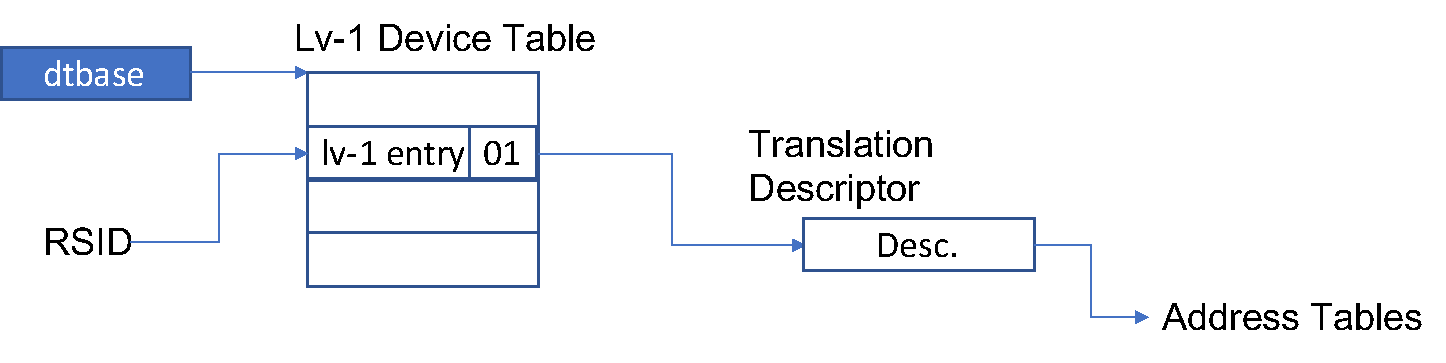
\includegraphics[width=0.95\textwidth]{img/dev_tbl_lookup_short_rsid.pdf}
    \caption{Device table look-up with only RSID and one stage of translation}
    \label{fig:dev_tbl_lookup_rsid_short}
\end{figure}

\begin{figure}[h!t]
    \centering
    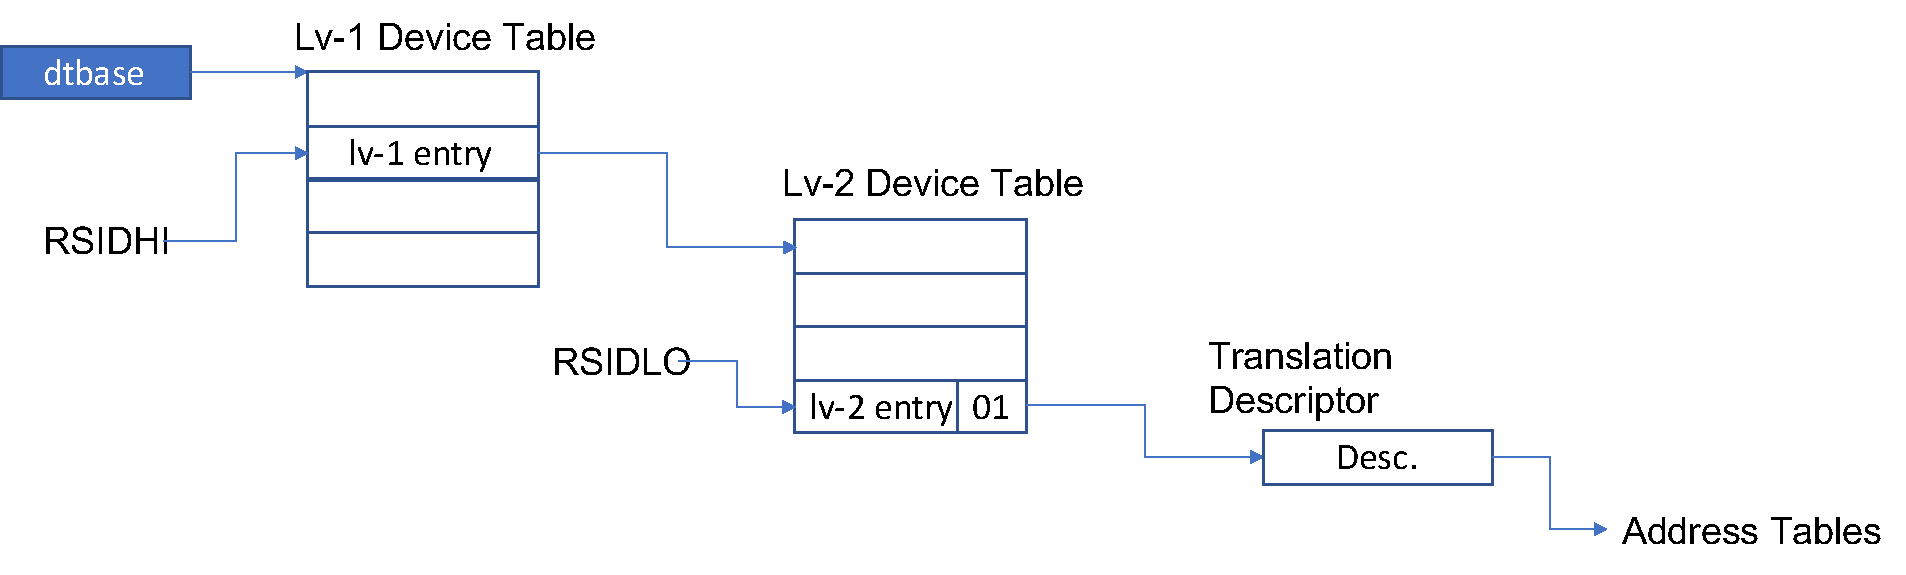
\includegraphics[width=0.95\textwidth]{img/dev_tbl_lookup_bare.pdf}
    \caption{Device table look-up with RSIDHI and RSIDLO and one stage of translation}
    \label{fig:dev_tbl_lookup_bare}
\end{figure}

\begin{figure}[h!t]
    \centering
    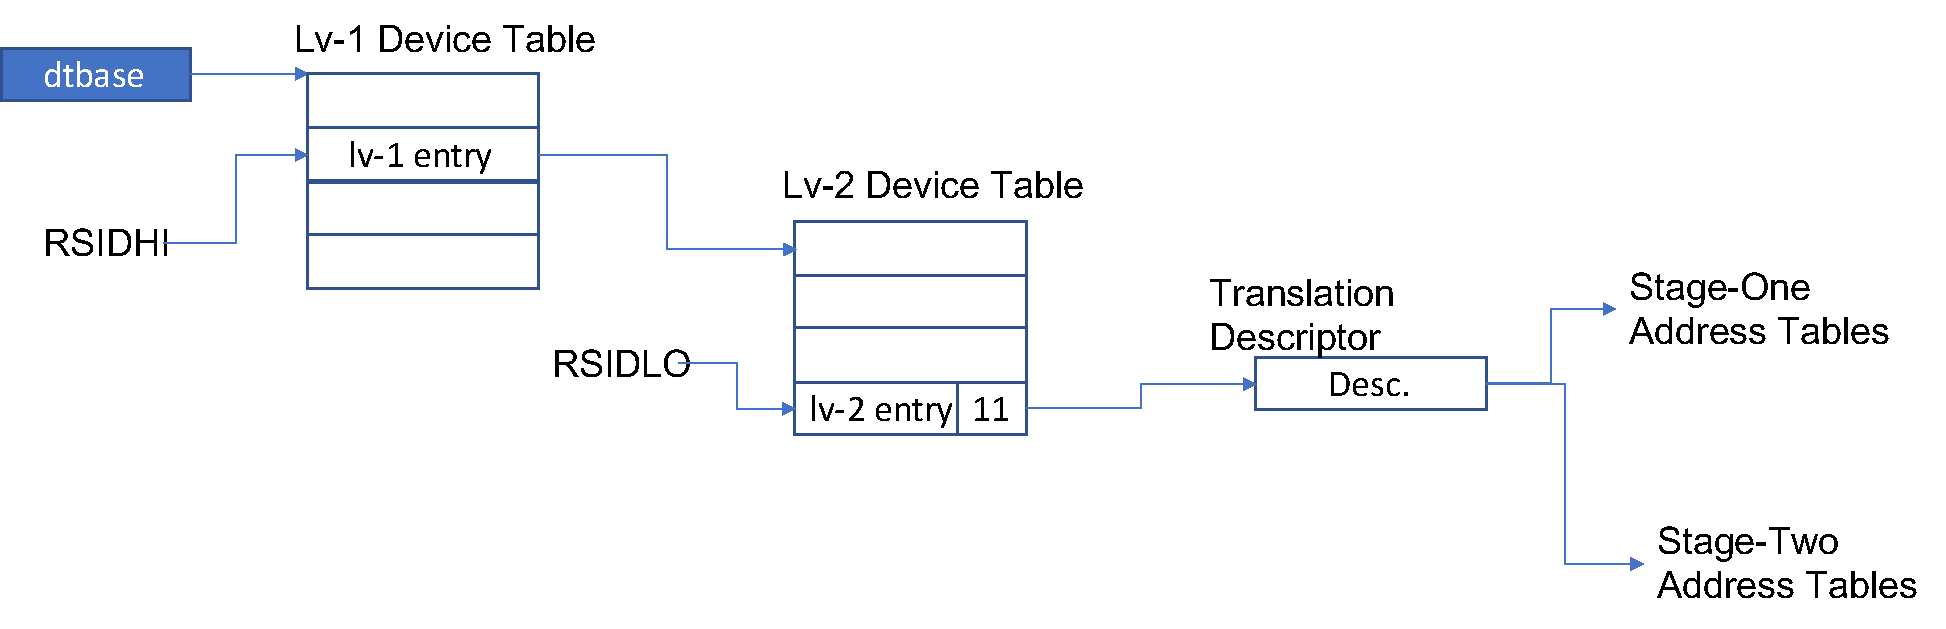
\includegraphics[width=0.95\textwidth]{img/dev_tbl_lookup_two_stage.pdf}
    \caption{Device table look-up when stage-two translation is used.}
    \label{fig:dev_tbl_lookup_two_stage}
\end{figure}

